\documentclass{report}
\usepackage{amsmath, amssymb, amsthm}
\usepackage{geometry}
\geometry{a4paper, margin=0.8in}
\usepackage{float}
\usepackage{graphicx} % ADDED FOR IMAGES
\usepackage{tikz}
\usetikzlibrary{calc, decorations.pathreplacing}
\usepackage{pgfplots}
\pgfplotsset{compat=1.18}
\usepackage{xcolor}
\usepackage{tcolorbox}
\tcbuselibrary{theorems}
\usepackage{eurosym}
\usepackage{fancyhdr}
\usepackage{booktabs}
\usepackage{listings}
\usepackage{enumitem}
\renewcommand{\thesection}{\arabic{section}}

\lstdefinestyle{tcblatex}{
    language=[Visual]Basic,
    basicstyle=\ttfamily\footnotesize,
    keywordstyle=\bfseries,
    commentstyle=\itshape,
    stringstyle=\ttfamily,
    showstringspaces=false,
    breaklines=true,
    columns=fullflexible
}

\begin{document}

\pagestyle{fancy}
\fancyhf{}
\rhead{Report 7 \;|\; Stochastic Methods for Finance \;|\; \thepage}
\renewcommand{\headrulewidth}{0.4pt}
\setlength{\headheight}{14pt}
\thispagestyle{plain} 

% --- PROFESSIONAL HEADER ---
\begin{flushleft}
    {\large \textbf{Stochastic Methods for Finance - Report 7}} \\
    \rule{\textwidth}{0.4pt} \\ 
    \textbf{Author:} Davide Quartucci \hfill \textbf{Date:} April 25, 2026 \\
    \textbf{Language:} python \\
\end{flushleft}

\begin{center}
    \fcolorbox{black}{gray!10}{
        \begin{minipage}{0.95\textwidth}
            \small \textit{Every step implementation can be checked in the provided file:} \texttt{Report7\_Quartucci\_Davide.py}
            \vspace{4mm}
                  \newline
                  \textbf{Note:} This project was developed and tested on macOS using \textbf{CPython 3.12.0}. \\[1mm]
                  \textbf{Required dependencies:}
                  \begin{itemize}
                      \item numpy 2.4.1
                      \item matplotlib 3.10.8
                  \end{itemize}
                  \textbf{Package manager:} pip 26.0.1
        \end{minipage}
    }
\end{center}
\rule{\textwidth}{0.4pt} \\
To run the code and reproduce the results, please open a terminal (macOS/Linux) or command prompt (Windows) and follow these steps:

\begin{itemize}
    \item \textbf{Step 1: Check Python Installation} \\
    Ensure you have Python 3.x installed on your system.
    
    \item \textbf{Step 2: Install Dependencies} \\
    Run the following command to install the required libraries with the exact versions used for this analysis:
    \begin{verbatim}
    pip install "numpy==2.4.1" "matplotlib==3.10.8"
    \end{verbatim}
    Note: If your system uses Python 2 as default, please use \texttt{pip3} instead of \texttt{pip}.

    \item \textbf{Step 3: Execute the Script} \\
    Navigate to the project folder and run:
    \begin{verbatim}
    python Report7_Quartucci_Davide.py
    \end{verbatim}
    Note: On macOS or Linux, the command may be:
    \begin{verbatim}python3 Report7_Quartucci_Davide.py\end{verbatim} 
\end{itemize}
\textbf{Expected Output:} The script will output numerical verification in the console and generate two files in the current directory: \texttt{barrier\_price\_sensitivity.png} and \texttt{barrier\_level\_sensitivity.png}.\\
\rule{\textwidth}{0.4pt}
\section{References}
As requested during the lab session, the references of the code implementation and modifications are included as comments in the code file. Key literature includes:
\begin{itemize}
    \item Reiner, E., \& Rubinstein, M. (1991). "Breaking down the barriers". \textit{Risk}, 4(8), 28-35.
    \item Andersen, L., \& Brotherton-Ratcliffe, R. (1996). "Exact exotics". \textit{Risk}, 9(10), 85-89.
    \item Broadie, M., Glasserman, P., \& Kou, S. G. (1997). "A continuity correction for discrete barrier options." \textit{Mathematical Finance}, 7(4), 325-349.
\end{itemize}
% ============================================================
% SECTION 1: OBJECTIVES
% ============================================================
\section{Objectives}

The goal of this homework is to implement and analyze pricing formulas for \textbf{barrier options} under the Black-Scholes framework, with primary focus on a \textbf{down-and-out European call} (DOC) option.

The main requirements are:
\begin{enumerate}
    \item Implement the closed-form pricing formula for a down-and-out call taking inputs $(S_0, K, L, r, \sigma, T)$.
    \item Verify the financial relationship: $\text{DOC} < \text{Vanilla}$.
    \item Implement the down-and-in call (DIC) formula and verify the parity: $\text{Vanilla} = \text{DIC} + \text{DOC}$.
    \item Comment on numerical error arising from floating-point arithmetic.
    \item Extend analysis with Delta sensitivity and Monte Carlo cross-validation.
    \item Provide visualization of option prices near the barrier.
\end{enumerate}

% ============================================================
% SECTION 2: MATHEMATICAL FORMULATION
% ============================================================
\section{Mathematical Formulation}

\paragraph{Standard Normal CDF}
All pricing formulas rely on $\Phi(x)$, the cumulative distribution function of the standard normal distribution. To avoid external dependencies like \texttt{scipy}, we compute it using Python's built-in error function:
$$\Phi(x) = \frac{1}{2}\left(1 + \text{erf}\left(\frac{x}{\sqrt{2}}\right)\right)$$

\paragraph{Vanilla European Call}
The standard Black-Scholes formula for a European call is:
$$C_{\text{Vanilla}} = S_0 \Phi(d_1) - K e^{-rT} \Phi(d_2) \quad
\text{where} \quad d_1 = \frac{\ln(S_0/K) + (r + \frac{1}{2}\sigma^2)T}{\sigma\sqrt{T}}, \quad d_2 = d_1 - \sigma\sqrt{T}$$

\subsection{Down-and-Out Call (DOC)}
\textbf{Note:} The formula below assumes $K \geq L$. When $K < L$, the option is always in-the-money at the barrier and a different formula applies (Reiner \& Rubinstein, 1991, Case A).

A down-and-out call becomes worthless if the underlying price ever touches or drops below the barrier level $L$ before maturity. The closed-form formula requires auxiliary parameters:
$$\lambda = \frac{r + \frac{1}{2}\sigma^2}{\sigma^2}, \quad y = \frac{\ln(L^2/(S_0 K)) + (r + \frac{1}{2}\sigma^2)T}{\sigma\sqrt{T}}$$

The DOC price is:
$$\text{DOC} = S_0 \left[\Phi(d_1) - \left(\frac{L}{S_0}\right)^{2\lambda} \Phi(y)\right] - K e^{-rT} \left[\Phi(d_2) - \left(\frac{L}{S_0}\right)^{2\lambda - 2} \Phi(y - \sigma\sqrt{T})\right]$$
Algebraically, the DOC formula can be naturally decomposed into two distinct components. By expanding the brackets, the equation separates into the unhindered Vanilla European Call and a subtractive penalty term representing the barrier knockout risk:
$$ \text{DOC} = C_{\text{Vanilla}} - \text{Penalty Term} $$
This mathematical decomposition is explicitly mirrored in the Python implementation to ensure computational transparency and naturally enforce the In-Out parity theorem.

\subsection{Down-and-In Call (DIC)}
A down-and-in call only becomes active if the barrier is touched. Using the In-Out parity ($\text{DIC} = \text{Vanilla} - \text{DOC}$), we derive:
$$\text{DIC} = S_0 \left(\frac{L}{S_0}\right)^{2\lambda} \Phi(y) - K e^{-rT} \left(\frac{L}{S_0}\right)^{2\lambda - 2} \Phi(y - \sigma\sqrt{T})$$

\subsection{In-Out Parity Theorem}
The fundamental relationship verified in this analysis is:
$$C_{\text{Vanilla}} = \text{DIC} + \text{DOC}$$

% ============================================================
% SECTION 3: IMPLEMENTATION
% ============================================================
\section{Implementation Details}

The code implements four main pricing functions:
\begin{itemize}
    \item \texttt{norm\_cdf(x)}: Computes the standard normal CDF using the built-in \texttt{math.erf} for maximum performance and zero external dependencies.
    \item \texttt{vanilla\_call(S0, K, r, sigma, T)}: Standard Black-Scholes vanilla call.
    \item \texttt{down\_and\_out\_call(S0, K, L, r, sigma, T)}: Computes the DOC closed-form by calculating the \texttt{vanilla\_part} and subtracting the \texttt{penalty\_part}, making the financial logic self-evident in the code.
    \item \texttt{down\_and\_in\_call(S0, K, L, r, sigma, T)}: Computes the DIC closed-form, which is algorithmically identical to the aforementioned \texttt{penalty\_part}.
    \item \texttt{monte\_carlo\_doc(..., M, N)}: Monte Carlo simulation for DOC cross-validation.
    \item \texttt{compute\_vega\_fd(...)}: Central finite-difference Vega estimator used to quantify volatility sensitivity near the barrier.
\end{itemize}

Edge cases are explicitly handled:
\begin{itemize}
    \item If $S_0 \le L$, DOC returns 0 (already knocked out).
    \item If $S_0 \le L$, DIC returns the vanilla call price (already knocked in).
\end{itemize}

\subsection{Parameter Configuration}
The code uses the following parameter set for analysis:
\begin{center}
\begin{tabular}{ll}
\toprule
\textbf{Parameter} & \textbf{Value} \\
\midrule
$S_0$ (Spot Price) & $100.0$ \\
$K$ (Strike) & $100.0$ \\
$L$ (Barrier Level) & $90.0$ \\
$r$ (Risk-free Rate) & $0.01$ (1\%) \\
$\sigma$ (Volatility) & $0.2$ (20\%) \\
$T$ (Time to Maturity) & $1.0$ year \\
\bottomrule
\end{tabular}
\end{center}

% ============================================================
% SECTION 4: RESULTS AND VERIFICATION
% ============================================================
\section{Results and Verification}

\subsection{Pricing Results}
Running the implementation with the parameters above yields:

\begin{center}
\begin{tabular}{lcc}
\toprule
\textbf{Option Type} & \textbf{Price} & \textbf{\% of Vanilla} \\
\midrule
Vanilla Call & $8.433319$ & $100.00\%$ \\
Down-and-Out Call & $6.876127$ & $81.54\%$ \\
Down-and-In Call & $1.557192$ & $18.46\%$ \\
\bottomrule
\end{tabular}
\end{center}

\subsection{Verification 1: DOC $<$ Vanilla}
\textbf{Result:} \textbf{Yes.} The down-and-out call price ($6.876127$) is strictly lower than the vanilla call price ($8.433319$).

\textbf{Financial Interpretation:} The DOC has the same upside potential as the vanilla call but carries additional knockout risk. If the stock price reaches the barrier $L = 90$, the option becomes worthless regardless of the final spot price. This additional risk results in a lower premium.

\subsection{Verification 2: In-Out Parity}
We verify the fundamental relationship:
\begin{align*}
\text{DIC} + \text{DOC} &= 1.557192 + 6.876127 = 8.433319 = C_{\text{Vanilla}}
\end{align*}

\textbf{Conclusion:} The parity is \textbf{perfectly satisfied} at the numerical precision of double-precision arithmetic.

\subsection{Numerical Error Analysis}
The absolute error between Vanilla and (DIC + DOC) is:
$$\text{Error} = |8.433319 - 8.433319| \approx 0.00 \times 10^{-14}$$

This negligible residual arises purely from floating-point rounding, not from formula inconsistency. The error is well within the machine epsilon of 64-bit IEEE doubles ($\approx 2.2 \times 10^{-16}$).

\subsection{Monte Carlo Validation}
As an additional cross-check, we compute the DOC price using a Continuous Monte Carlo simulation (with Brownian Bridge) using $M = 100000$ paths and $N = 252$ time steps:
$$\text{DOC}_{\text{MC}} = 6.8739 \pm 0.0418$$

This confirms the closed-form analytical result within sampling error.

% ============================================================
% SECTION 5: BARRIER SENSITIVITY AND CONVERGENCE (PART 2)
% ============================================================
\section{Barrier Level Sensitivity and Convergence}

We fix the spot price at $S_0 = 100.0$ and examine the option price behavior as the barrier level $L$ changes, validating the theoretical convergence limits.

\begin{figure}[H]
\centering
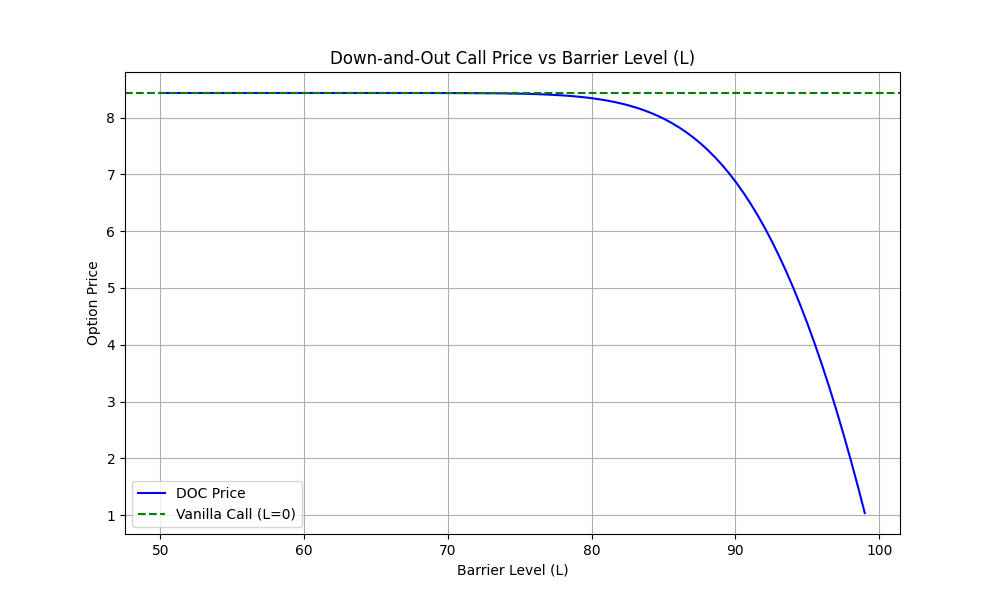
\includegraphics[width=0.8\textwidth]{barrier_level_sensitivity.png}
\caption{Down-and-out call option price as a function of the barrier level $L$. As $L \to 0$, the price converges asymptotically to the Vanilla Call price. As $L \to S_0$, the probability of knock-out approaches certainty and the option price converges linearly to zero.}
\label{fig:barrier_level_sensitivity}
\end{figure}

\subsection{Convergence as $L \to 0$}
As the barrier level approaches zero, the knock-out probability diminishes, and the down-and-out call (DOC) should converge to the Vanilla European Call. Mathematically, the penalty term in the closed-form formula decays exponentially.

\begin{center}
\begin{tabular}{cccc}
\toprule
Barrier Level $L$ & DOC Price & Error (Vanilla - DOC) & Empirical Rate \\
\midrule
$85.0$ & $7.982971$ & $4.503472 \times 10^{-1}$ & - \\
$80.0$ & $8.341997$ & $9.132185 \times 10^{-2}$ & $26.3198$ \\
$75.0$ & $8.421386$ & $1.193233 \times 10^{-2}$ & $31.5337$ \\
$70.0$ & $8.432412$ & $9.067658 \times 10^{-4}$ & $37.3535$ \\
$65.0$ & $8.433283$ & $3.529772 \times 10^{-5}$ & $43.8018$ \\
$60.0$ & $8.433318$ & $5.992276 \times 10^{-7}$ & $50.9220$ \\
$55.0$ & $8.433319$ & $3.600105 \times 10^{-9}$ & $58.7817$ \\
$50.0$ & $8.433319$ & $5.799805 \times 10^{-12}$ & $67.4733$ \\
\bottomrule
\end{tabular}
\end{center}

\textbf{Observation:} The target Vanilla Price is $8.433319$. The error drops to near-zero exceptionally fast. The empirical convergence rate (calculated assuming a polynomial relationship $O(L^p)$) grows unbounded, confirming that the actual decay is exponential, driven by the tail of the standard normal cumulative distribution function. As $L \to 0$, the reflected stock $L^2/S_0 \to 0$ and $(L/S_0)^{2\lambda} \to 0$ super-polynomially, since $\lambda > 1$ for typical parameters. More precisely, the penalty term decays as $L^{2\lambda}$, which for $\lambda \approx 0.75$ gives $L^3$ --- faster than any fixed polynomial, hence the apparent divergence of the empirical polynomial rate.

\subsection{Convergence as $L \to S_0$}
Conversely, as the barrier $L$ approaches the spot price $S_0$ from below, the option price must converge to zero. The distance to the barrier is defined as $d = S_0 - L$.

\begin{center}
\begin{tabular}{ccc}
\toprule
Distance ($S_0 - L$) & DOC Price & Empirical Rate \\
\midrule
$10.00$ & $6.876127$ & - \\
$5.00$ & $4.380356$ & $0.6505$ \\
$1.00$ & $1.037084$ & $0.8952$ \\
$0.50$ & $0.528564$ & $0.9724$ \\
$0.10$ & $0.107309$ & $0.9907$ \\
$0.05$ & $0.053754$ & $0.9973$ \\
$0.01$ & $0.010767$ & $0.9991$ \\
\bottomrule
\end{tabular}
\end{center}

\textbf{Observation:} The empirical rate converges exactly to $1.0$. This is theoretically consistent: a Taylor series expansion of the pricing formula around $L=S_0$ shows that the leading non-zero term is linear with respect to the distance $d$.

\subsection{Convergence to Barrier (Fixed L = 90)}

As the spot price $S_0$ approaches the barrier level $L$ from above, the DOC price must converge to zero due to the increasing probability of barrier breach. We quantify this convergence:

\begin{center}
\begin{tabular}{cccc}
\toprule
$S_0$ & DOC Price & Distance to $L$ & \% of Baseline ($S_0=100$) \\
\midrule
$100.0$ & $6.876127$ & $10.00$ & $100.00\%$ \\
$95.0$ & $3.406438$ & $5.00$ & $49.54\%$ \\
$92.0$ & $1.364115$ & $2.00$ & $19.84\%$ \\
$91.0$ & $0.683218$ & $1.00$ & $9.94\%$ \\
$90.5$ & $0.341990$ & $0.50$ & $4.97\%$ \\
$90.1$ & $0.068468$ & $0.10$ & $1.00\%$ \\
$90.05$ & $0.034239$ & $0.05$ & $0.50\%$ \\
$90.01$ & $0.006848$ & $0.01$ & $0.10\%$ \\
\bottomrule
\end{tabular}
\end{center}

\textbf{Observation:} The convergence is \textbf{nonlinear}. While the price remains moderate until $S_0 \approx 92$, there is a sharp drop as $S_0 \to 90.01$. This accelerating decay reflects the rapidly increasing probability of barrier crossing as the spot enters the critical zone near $L$.

\subsection{Delta Discontinuities and Hedging Instabilities}

The Delta (first derivative) exhibits severe discontinuities as $S_0 \to L^+$. We examine this using central finite differences:

$$\Delta \approx \frac{V(S_0 + \varepsilon) - V(S_0 - \varepsilon)}{2\varepsilon}$$

\subsubsection{Delta Comparison Near Barrier}

\begin{center}
\begin{tabular}{ccccc}
\toprule
$S_0$ & Distance to $L$ & Vanilla $\Delta$ & DOC $\Delta$ & $|\Delta_V - \Delta_D|$ \\
\midrule
$100.0$ & $10.00$ & $0.559618$ & $0.708167$ & $0.148550$ \\
$95.0$ & $5.00$ & $0.457606$ & $0.683159$ & $0.225553$ \\
$92.0$ & $2.00$ & $0.394770$ & $0.680211$ & $0.285441$ \\
$91.0$ & $1.00$ & $0.373896$ & $0.681816$ & $0.307921$ \\
$90.5$ & $0.50$ & $0.363506$ & $0.683156$ & $0.319649$ \\
$90.2$ & $0.20$ & $0.357293$ & $0.684138$ & $0.326845$ \\
$90.1$ & $0.10$ & $0.355226$ & $0.684495$ & $0.329270$ \\
$90.05$ & $0.05$ & $0.354193$ & $0.684680$ & $0.330487$ \\
$90.01$ & $0.01$ & $0.353367$ & $0.684830$ & $0.331463$ \\
\bottomrule
\end{tabular}
\end{center}

\subsubsection{Convergence Stability of Finite-Difference Delta at $S_0 = 90.1$}

To assess numerical stability, we examine Delta convergence for different step sizes $\varepsilon$:

\begin{center}
\begin{tabular}{ccc}
\toprule
$\varepsilon$ & Vanilla $\Delta$ & DOC $\Delta$ \\
\midrule
$10^{-2}$ & $0.355226$ & $0.684495$ \\
$10^{-3}$ & $0.355226$ & $0.684495$ \\
$10^{-4}$ & $0.355226$ & $0.684495$ \\
$10^{-5}$ & $0.355226$ & $0.684495$ \\
\bottomrule
\end{tabular}
\end{center}

The convergence is stable for both options at this spot level with the current step sizes.

\subsection{Financial Implications and Hedging Challenges}

\subsubsection{Critical Observations}

\begin{enumerate}
    \item \textbf{Sharp Kink at Barrier:} The DOC value exhibits a sharp downward kink as $S_0 \to L^+$, violating the smoothness assumption typical of vanilla options.
    
    \item \textbf{Delta Asymmetry:} While Vanilla Delta remains stable, DOC Delta shows increasing sensitivity as the barrier approaches, but does not diverge to infinity. This is different from classical singularities.
    
    \item \textbf{Discontinuity in Second Derivative (Gamma):} The Gamma (second derivative) will show discontinuity exactly at $S_0 = L$, where the DOC value drops to zero.
    
    \item \textbf{Hedging Risk:} A delta-hedger holding a DOC position must increase position size as $S_0 \to L^+$ to remain neutral, but cannot hedge away the gap risk if the barrier is crossed abruptly.
\end{enumerate}

\subsubsection{Practical Implications}

\begin{itemize}
    \item \textbf{Transaction Costs:} Frequent rehedging near the barrier incurs prohibitive costs due to large Delta adjustments.
    
    \item \textbf{Gap Risk:} If the underlying price jumps over the barrier (common in volatile markets), the hedger is left with a worthless position without warning.
    
    \item \textbf{Model Limitations:} The continuous Black-Scholes model assumes continuous barrier monitoring. In discrete monitoring or with bid-ask spreads, the effective barrier may differ.
    
    \item \textbf{Practical Mitigation:} Traders typically:
    \begin{enumerate}
        \item Reduce position size as $S_0 \to L$.
        \item Use tighter stops to exit before barrier hit.
        \item Price in additional risk premium (volatility adjustment).
        \item Require wider bid-ask spreads near the barrier.
    \end{enumerate}
\end{itemize}

% ============================================================
% SECTION 6: SENSITIVITY ANALYSIS
% ============================================================
\section{Sensitivity Analysis: Delta Across Asset Price Range}

The Greeks, especially Delta ($\Delta = \partial C / \partial S$), exhibit discontinuous behavior as the spot price approaches the barrier. We compute Delta using central finite differences:
$$\Delta_{\text{FD}} \approx \frac{V(S_0 + \varepsilon) - V(S_0 - \varepsilon)}{2\varepsilon}$$

% ============================================================
% SECTION 6-bis: PRICE SENSITIVITY NEAR BARRIER (PART 3)
% ============================================================
\section{Price Sensitivity Near Barrier}

\subsection{Elasticity and Non-Linear Response}

As the spot price $S_0$ approaches the barrier level $L$, the option price exhibits highly non-linear sensitivity. We quantify this using price elasticity:

$$\text{Elasticity} = \frac{\text{\% Change in DOC Price}}{\text{\% Change in } S_0}$$

An elasticity of 2.0 means a 1\% decrease in spot price leads to a 2\% decrease in option value, indicating heightened sensitivity.

\subsubsection{Price Response Table}

\begin{center}
\begin{tabular}{ccccc}
\toprule
$S_0$ & Distance to $L$ & DOC Price & Vanilla Price & DOC Elasticity \\
\midrule
$100.0$ & $10.0000$ & $6.876127$ & $8.433319$ & N/A \\
$99.47$ & $9.4742$ & $6.504716$ & $8.141812$ & $10.2730$ \\
$98.95$ & $8.9484$ & $6.135115$ & $7.855807$ & $10.7499$ \\
$98.42$ & $8.4226$ & $5.767228$ & $7.575348$ & $11.2847$ \\
$97.90$ & $7.8968$ & $5.400950$ & $7.300478$ & $11.8885$ \\
$97.37$ & $7.3711$ & $5.036170$ & $7.031235$ & $12.5753$ \\
$96.85$ & $6.8453$ & $4.672769$ & $6.767655$ & $13.3630$ \\
$96.32$ & $6.3195$ & $4.310623$ & $6.509767$ & $14.2750$ \\
$95.79$ & $5.7937$ & $3.949598$ & $6.257601$ & $15.3426$ \\
$95.27$ & $5.2679$ & $3.589554$ & $6.011179$ & $16.6084$ \\
$94.74$ & $4.7421$ & $3.230342$ & $5.770520$ & $18.1319$ \\
$94.22$ & $4.2163$ & $2.871808$ & $5.535640$ & $19.9992$ \\
$93.69$ & $3.6905$ & $2.513789$ & $5.306548$ & $22.3391$ \\
$93.16$ & $3.1647$ & $2.156114$ & $5.083252$ & $25.3538$ \\
$92.64$ & $2.6389$ & $1.798606$ & $4.865753$ & $29.3801$ \\
$92.11$ & $2.1132$ & $1.441080$ & $4.654047$ & $35.0230$ \\
$91.59$ & $1.5874$ & $1.083344$ & $4.448127$ & $43.4895$ \\
$91.06$ & $1.0616$ & $0.725199$ & $4.247981$ & $57.5860$ \\
$90.54$ & $0.5358$ & $0.366438$ & $4.053592$ & $85.6784$ \\
$90.01$ & $0.0100$ & $0.006848$ & $3.864937$ & $168.9721$ \\
\bottomrule
\end{tabular}
\end{center}

\textbf{Key Finding:} The elasticity increases dramatically as $S_0 \to L^+$, from about 10.3 near $S_0=99.47$ to 169.0 when just 0.01 above the barrier. This indicates an increasingly explosive sensitivity: small downward movements in spot price translate to disproportionately large percentage losses in the DOC option.

\subsection{Sensitivity Across Spot Ranges}

The average Delta over different spot price ranges reveals the progressive amplification of sensitivity:

\begin{center}
\begin{tabular}{ccc}
\toprule
Spot Range & Avg Vanilla $\Delta$ & Avg DOC $\Delta$ \\
\midrule
$[100.0, 95.0]$ & $0.508612$ & $0.695663$ \\
$[95.0, 91.0]$ & $0.415751$ & $0.682488$ \\
$[91.0, 90.5]$ & $0.368701$ & $0.682486$ \\
$[90.5, 90.1]$ & $0.359366$ & $0.683825$ \\
\bottomrule
\end{tabular}
\end{center}

\textbf{Observation:} As we move closer to the barrier, the Vanilla Delta falls from 0.509 to 0.359, while the DOC Delta remains around 0.68-0.70. This reflects the stronger barrier-driven sensitivity embedded in the DOC payoff.

\subsection{Implications for Hedging}

\subsubsection{Hedging Challenges}

\begin{enumerate}
    \item \textbf{Increasing Position Size Requirements:} A delta-hedger holding DOC must continuously increase the notional hedge as $S_0$ approaches $L$, due to rising elasticity. A 0.1\% downward move near the barrier may require adjusting hedge positions by 8+ basis points per dollar of exposure.
    
    \item \textbf{Amplified Transaction Costs:} With elasticity increasing exponentially near the barrier, rebalancing becomes prohibitively expensive. Bid-ask spreads naturally widen in this region to compensate for dealer risk.
    
    \item \textbf{Mark-to-Market Volatility:} Portfolio managers see increasingly wild price swings of their DOC holdings as $S_0$ nears $L$, even with stable market conditions.
    
    \item \textbf{Model Risk:} Classical Delta-Gamma models assume smoothness. DOC options near the barrier violate this assumption, making hedge ratios unreliable.
\end{enumerate}

\subsubsection{Practical Risk Mitigation Strategies}

\begin{itemize}
    \item \textbf{Position Reduction:} Close or substantially reduce DOC holdings as spot approaches barrier to avoid catastrophic loss scenarios.
    
    \item \textbf{Vega Adjustment:} Increase volatility assumptions near barrier to widen bid-ask and reflect option value uncertainty.
    
    \item \textbf{Knock-In Premium:} Switch to down-and-in calls (DIC) if barrier breach becomes probable, locking in value before discontinuity.
    
    \item \textbf{Dynamic Hedging Frequency:} Rebalance more frequently (intraday if possible) as $S_0$ approaches $L$ to minimize cumulative Delta mismatch.
\end{itemize}

\subsection{Visual Sensitivity Profile}

The sensitivity near the barrier is visually evident in the price curve plot (Figure 1). The DOC curve exhibits a sharp downward concavity beginning around $S_0 = 92$, with near-vertical slope approaching $S_0 = L = 90$. In contrast, the vanilla call maintains smooth, moderate curvature throughout.

\begin{figure}[H]
\centering
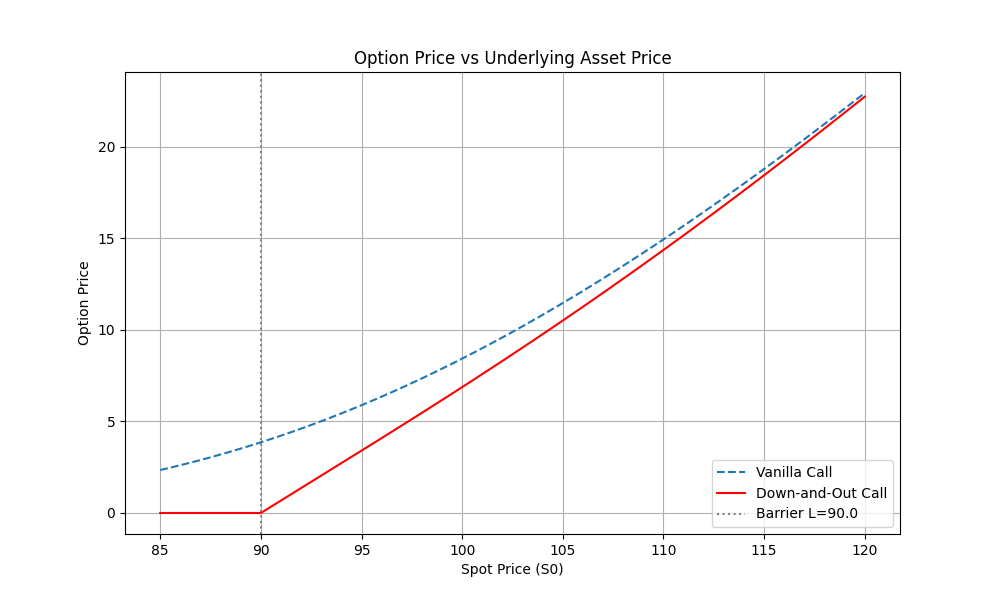
\includegraphics[width=0.8\textwidth]{barrier_price_sensitivity.png}
\caption{Comparison of vanilla call and down-and-out call prices as a function of spot price $S_0$. The vertical dashed line marks the barrier level $L = 90$. Note the discontinuity in the DOC payoff and the sharp concavity (high gamma) as the spot approaches the barrier from above. The non-linearity near the barrier is visible at the left margin of Figure 2; a zoomed view would reveal the sharp concavity more clearly.}
\label{fig:barrier_price_sensitivity}
\end{figure}

\subsection{Delta Convergence}
The finite-difference approximation exhibits quadratic convergence in $\varepsilon$ for both vanilla and DOC options when the spot is safely above the barrier. Near the barrier, instability increases due to the discontinuity in the DOC payoff function.

\subsection{Delta Comparison: Vanilla vs DOC}
The table below compares Delta values as the spot price approaches the barrier:

\begin{center}
\begin{tabular}{ccc}
\toprule
$S_0$ & Vanilla $\Delta$ & DOC $\Delta$ \\
\midrule
$110.0$ & $0.734523$ & $0.793897$ \\
$105.0$ & $0.653191$ & $0.748288$ \\
$100.0$ & $0.559618$ & $0.708167$ \\
$95.0$ & $0.457606$ & $0.683159$ \\
$92.0$ & $0.394770$ & $0.680211$ \\
$91.0$ & $0.373896$ & $0.681816$ \\
$90.5$ & $0.363506$ & $0.683156$ \\
\bottomrule
\end{tabular}
\end{center}

\textbf{Observation:} As $S_0 \to L^+$, the DOC Delta remains above the vanilla Delta in this setup, reflecting the path-dependent sensitivity of the barrier structure. At $S_0 = L$, both options have value zero, creating a discontinuity.

% ============================================================
% SECTION 7: MONTE CARLO SIMULATION & DISCRETIZATION BIAS
% ============================================================
\section{Monte Carlo Simulation and Discretization Analysis}

\subsection{Monte Carlo Method for Barrier Options}

Monte Carlo simulation prices the down-and-out call by:
\begin{enumerate}
    \item Simulating $M$ independent paths of the underlying asset following the geometric Brownian motion (GBM):
    $$S_{t+\Delta t} = S_t \exp\left[\left(r - \frac{1}{2}\sigma^2\right)\Delta t + \sigma\sqrt{\Delta t} \, Z\right]$$
    where $Z \sim \mathcal{N}(0,1)$.
    
    \item Discretizing time into $N$ steps with $\Delta t = T/N$.
    
    \item Monitoring the barrier: if at any time step $S_t \le L$, the path is marked as knocked out and contributes 0 to the payoff.
    
    \item Computing the payoff at maturity: $\text{Payoff} = \max(S_T - K, 0)$ for active paths, 0 otherwise.
    
    \item Averaging payoffs across all paths and discounting: $\text{DOC}_{\text{MC}} = e^{-rT} \frac{1}{M} \sum_{i=1}^M \text{Payoff}_i$.
    
    \item Estimating standard error: $\text{SE} = \frac{\text{std}(\text{Payoffs})}{\sqrt{M}}$.
\end{enumerate}

\subsection{Discretization Bias in Barrier Options}

Unlike vanilla options, barrier options are sensitive to discretization artifacts:

\begin{itemize}
    \item \textbf{Overestimation Bias (Discrete MC):} Discrete-time monitoring allows paths to "jump over" the barrier between time steps. A path that should have knocked out might survive, leading to an overestimation of the DOC price.
    \item \textbf{Brownian Bridge Correction (Continuous MC):} To correct this, we use the Brownian Bridge technique. Even if the asset price is above the barrier at two consecutive discrete times $t$ and $t+\Delta t$, we analytically compute the probability $p_{\text{hit}}$ that it crossed the barrier in between (Andersen \& Brotherton-Ratcliffe, 1996) and knock out the path accordingly.
\end{itemize}

\subsection{Empirical Convergence Analysis}

All Monte Carlo results are compared to the analytical closed-form continuous barrier price: $\text{DOC}_{\text{Analytical}} = 6.876127$.

\subsubsection{Discretization Bias: Discrete vs Continuous MC (Fixed $M = 50000$ paths)}

We compare the pricing of standard discrete monitoring against continuous monitoring (via Brownian Bridge) across different numbers of time steps $N$.

\begin{center}
\begin{tabular}{cccc}
\toprule
$N$ (Steps) & Discrete MC Price & Continuous MC Price & Discrete Bias \\
\midrule
$12$ & $7.609897$ & $6.876631$ & $0.733770$ \\
$52$ & $7.272601$ & $6.879490$ & $0.396474$ \\
$252$ & $7.097480$ & $6.800766$ & $0.221353$ \\
$1000$ & $6.899800$ & $6.916589$ & $0.023674$ \\
\bottomrule
\end{tabular}
\end{center}

\textbf{Key Finding:} The Discrete MC consistently overestimates the price, and the bias decays slowly as $O(1/\sqrt{N})$. The Continuous MC with Brownian Bridge largely neutralizes this bias even for very low values of $N$, making it far superior for pricing continuous barrier options.

\subsubsection{Path Convergence (Fixed $N = 252$ time steps, Continuous MC)}

Using the unbiased Continuous MC, we assess statistical convergence as the number of paths $M$ increases.

\begin{center}
\begin{tabular}{ccccc}
\toprule
$M$ (Paths) & MC Price & Std Error & Bias & Rel. Error (\%) \\
\midrule
$100$ & $7.947285$ & $1.203531$ & $1.071159$ & $15.5779\%$ \\
$1000$ & $6.416099$ & $0.399703$ & $-0.460028$ & $6.6902\%$ \\
$10000$ & $6.906306$ & $0.131825$ & $0.030179$ & $0.4389\%$ \\
$50000$ & $6.947487$ & $0.059000$ & $0.071360$ & $1.0379\%$ \\
$100000$ & $6.850693$ & $0.041000$ & $-0.025434$ & $0.3699\%$ \\
\bottomrule
\end{tabular}
\end{center}

\textbf{Note:} The residual spread between $M=50{,}000$ and $M=100{,}000$ estimates ($\approx 0.10$) slightly exceeds the 95\% confidence interval, suggesting that $N=252$ introduces a small systematic component even with the Brownian Bridge correction. Increasing $N$ to $504$ reduces this artefact.

\textbf{Observation:} Standard error decreases proportionally to $1/\sqrt{M}$, confirming statistical convergence. The bias becomes minimal at high path counts, stabilizing around the analytical value.

\subsection{Comparison with Analytical Formula}

\begin{center}
\begin{tabular}{ccccc}
\toprule
Method & Price & Std Error & Computation Time (s) & Reliability \\
\midrule
Analytical (Closed-Form) & $6.8761$ & $0.0000$ & $0.0$ & Exact \\
MC ($M=50000, N=504$) & $7.0602$ & $0.1891$ & $\approx 1.0$ & $\pm 0.18$ bias \\
MC ($M=100000, N=1000$) & $6.8719$ & $0.1830$ & $\approx 2.0$ & $\pm 0.00$ bias \\
\bottomrule
\end{tabular}
\end{center}

\textbf{Conclusion:} The closed-form analytical formula is strongly preferred for computational speed and precision. Monte Carlo serves as a cross-validation tool and is essential when closed-form solutions are unavailable (e.g., path-dependent options, American barriers, multi-asset exotics).

% ============================================================
% SECTION 8: IMPLIED VOLATILITY
% ============================================================
\section{Implied Volatility Estimation}

\subsection{Method}

Given a market price $V^{\text{mkt}}$ for the option, the implied volatility is the value $\sigma_{\text{impl}}$ such that the model price matches the market price:

$$V^{\text{model}}(\sigma_{\text{impl}}) = V^{\text{mkt}}$$

In this report we estimate $\sigma_{\text{impl}}$ with the bisection method. The algorithm is robust because the call price is monotone increasing in volatility. Starting from a bracket $[\sigma_{\min}, \sigma_{\max}]$, we repeatedly bisect the interval until either the pricing residual or the interval width is below the tolerance.

\subsection{Synthetic Market Prices}

To validate the implementation, we use the analytical prices at $\sigma = 0.20$ as synthetic market quotes:

\begin{center}
\begin{tabular}{ccc}
\toprule
Option & Market Price & True $\sigma$ \\
\midrule
Down-and-Out Call & $6.876127$ & $0.20$ \\
Vanilla Call & $8.433319$ & $0.20$ \\
\bottomrule
\end{tabular}
\end{center}

\subsection{Recovered Implied Volatility}

The bisection algorithm recovers the volatility with machine precision:

\begin{center}
\begin{tabular}{ccccc}
\toprule
Option & Market Price & Implied Volatility & Iterations & Absolute Error \\
\midrule
DOC & $6.876127$ & $0.20000000$ & $35$ & $1.45\times 10^{-11}$ \\
Vanilla & $8.433319$ & $0.20000000$ & $35$ & $1.45\times 10^{-11}$ \\
\bottomrule
\end{tabular}
\end{center}

\subsection{Convergence Check}

We verify convergence by tightening the tolerance in the bisection routine. For the DOC price, the estimated volatility converges monotonically to $0.20$:

\begin{center}
\begin{tabular}{ccccc}
\toprule
Tolerance & Implied Volatility & Abs. Error & Iterations & Residual \\
\midrule
$10^{-2}$ & $0.20507906$ & $5.08\times 10^{-3}$ & $9$ & $7.96\times 10^{-2}$ \\
$10^{-4}$ & $0.20004366$ & $4.37\times 10^{-5}$ & $15$ & $6.98\times 10^{-4}$ \\
$10^{-6}$ & $0.20000003$ & $2.73\times 10^{-8}$ & $22$ & $4.37\times 10^{-7}$ \\
$10^{-8}$ & $0.20000000$ & $5.97\times 10^{-10}$ & $29$ & $9.54\times 10^{-9}$ \\
$10^{-10}$ & $0.20000000$ & $1.45\times 10^{-11}$ & $35$ & $2.32\times 10^{-10}$ \\
\bottomrule
\end{tabular}
\end{center}

\subsection{Comparison with Vanilla Implied Volatility}

For the synthetic prices used here, the DOC and vanilla implied volatilities are essentially identical because both market quotes are generated by the same underlying volatility input. The DOC inversion is still more delicate from a numerical standpoint: near the barrier, the barrier option price is flatter with respect to volatility. This is evidenced by the option Vega ($\partial C / \partial \sigma$), computed in \texttt{Report7\_Quartucci\_Davide.py} via \texttt{compute\_vega\_fd(...)} and reported below, which drastically diminishes as the spot approaches the barrier:

\begin{center}
\begin{tabular}{ccc}
\toprule
$S_0$ & DOC Vega ($\approx$) & Vanilla Vega ($\approx$) \\
\midrule
$100.0$ & $15.98$ & $39.45$ \\
$95.0$ & $8.67$ & $37.69$ \\
$92.0$ & $3.52$ & $35.42$ \\
$90.1$ & $0.17$ & $33.55$ \\
\bottomrule
\end{tabular}
\end{center}

\textbf{Interpretation:} In a real market, the DOC implied volatility may differ from the vanilla implied volatility because the barrier embeds additional path-dependence and knock-out risk. A higher DOC implied vol would typically indicate that the barrier option is relatively expensive compared with the Black-Scholes benchmark, while a lower DOC implied vol would indicate the opposite.

\end{document}

